\section{Лабараторная работа №1}

Для дадзенай работы неабходна скачаць драйвер для падключэння да
базы даных Mariadb (\textit{mariadb-java-client-1.1.10.jar}) і
пакласці ў \textit{WebContent/WEB-INF/lib}.

\subsection{Структура праекта}

На малюнку \ref{img: lab1} прадстаўлена файлавая структура праекта.

\begin{figure}[h!]
    \centering
    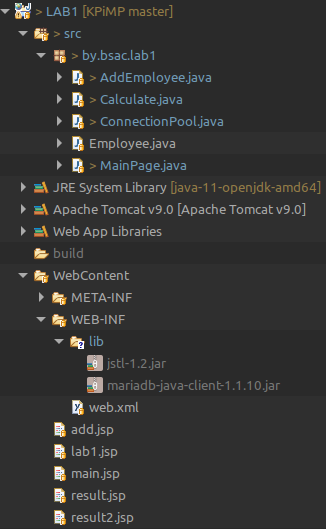
\includegraphics[width=0.5\textwidth]{lab1_structure}
    \caption{Файлавая структура практычнага занятку}
    \label{img: lab1} 
\end{figure}

\subsection{Заданне}

Стварыць вэб-праграму, якая дае магчымасць пошуку і прагляду супрацоўнікаў,
дабаўленне новага супрацоўніка.
Калі ў полі ўводу не было ўведзена імён, неабходна вывесці спіс
усіх супрацоўнікаў.
Інфармацыя пра супрацоўнікаў павінна захоўвацца ў базе даных.

\textit{Індывідуальнае заданне}: стварыць вэб-праграму, якая
будзе вылічваць значэнне трыганаметрычных функцый (выбар функцыі
ажыццяўляць пры дапамозе выпадаючага спісу).

\subsubsection{Старонка add.jsp}

У лістынгу \ref{lst: lab1_add.jsp} прадстаўлена старонка 
\textit{add.jsp}.

\lstinputlisting[caption={Старонка add.jsp},%
                 label={lst: lab1_add.jsp},%
                 language=HTML5,%
                 style=htmlcssjs]{LAB1/JSP/add.jsp}

\subsubsection{Старонка lab1.jsp}

У лістынгу \ref{lst: lab1_lab1.jsp} прадстаўлена старонка 
\textit{lab1.jsp}.

\lstinputlisting[caption={Старонка lab1.jsp},%
                 label={lst: lab1_lab1.jsp},%
                 language=HTML5,%
                 style=htmlcssjs]{LAB1/JSP/lab1.jsp}

\subsubsection{Старонка main.jsp}

У лістынгу \ref{lst: lab1_main.jsp} прадстаўлена старонка 
\textit{main.jsp}.

\lstinputlisting[caption={Старонка main.jsp},%
                 label={lst: lab1_main.jsp},%
                 language=HTML5,%
                 style=htmlcssjs]{LAB1/JSP/main.jsp}

\subsubsection{Старонка result.jsp}

У лістынгу \ref{lst: lab1_result.jsp} прадстаўлена старонка 
\textit{result.jsp}.

\lstinputlisting[caption={Старонка result.jsp},%
                 label={lst: lab1_result.jsp},%
                 language=HTML5,%
                 style=htmlcssjs]{LAB1/JSP/result.jsp}

\subsubsection{Старонка result2.jsp}

У лістынгу \ref{lst: lab1_result2.jsp} прадстаўлена старонка 
\textit{result2.jsp}.

\lstinputlisting[caption={Старонка result2.jsp},%
                 label={lst: lab1_result2.jsp},%
                 language=HTML5,%
                 style=htmlcssjs]{LAB1/JSP/result2.jsp}

\subsubsection{Клас AddEmployee.}

Дадзены клас адказвае за дабаўленне новага супрацоўніка ў базу даных.

У лістынгу \ref{lst: lab1_AddEmployee} прадстаўлены клас
\textit{AddEmployee}.

\lstinputlisting[caption={Клас AddEmployee},%
                 label={lst: lab1_AddEmployee},%
                 language=java]{LAB1/Java/AddEmployee.java}

\subsubsection{Клас Calculate.}

Дадзены клас (неабходны для індывідуальнага задання) вылічвае
трыганаметрычныя функцыі.

У лістынгу \ref{lst: lab1_Calculate} прадстаўлены клас
\textit{Calculate}.

\lstinputlisting[caption={Клас Calculate},%
                 label={lst: lab1_Calculate},%
                 language=java]{LAB1/Java/Calculate.java}

\subsubsection{Клас ConnectionPool.}

Дадзены клас неабходны для падключэння праграмы да базы даных.

У лістынгу \ref{lst: lab1_ConnectionPool} прадстаўлены клас
\textit{ConnectionPool}.

\lstinputlisting[caption={Клас ConnectionPool},%
                 label={lst: lab1_ConnectionPool},%
                 language=java]{LAB1/Java/ConnectionPool.java}

\subsubsection{Клас Employee.}

Дадзены клас захоўвае інфармацыю пра супрацоўнікаў.

У лістынгу \ref{lst: lab1_Employee} прадстаўлены клас
\textit{Employee}.

\lstinputlisting[caption={Клас Employee},%
                 label={lst: lab1_Employee},%
                 language=java]{LAB1/Java/Employee.java}

\subsubsection{Клас MainPage.}

Дадзены клас забяспечваю логіку галоўнай старонкі вэб-праграмы
(увод імя супрацоўніка для пошуку ў базе даных).

У лістынгу \ref{lst: lab1_MainPage} прадстаўлены клас
\textit{MainPage}.

\lstinputlisting[caption={Клас MainPage},%
                 label={lst: lab1_MainPage},%
                 language=java]{LAB1/Java/MainPage.java}
